%!TEX root = thesis.tex
\section{Introduction}
\section{Lake-Analyzer}
\section{Foundations}
\section{Matlab WPS}
	\begin{itemize}
		\item weakly typed language
		\item functions with multiple return values
		\item previous approaches: WPS4R
		\begin{itemize}
			\item heavily format specific
			\begin{itemize}
				\item parsing of GML/etc in the WPS and translation to R structures
				\item configuration as comments in R scripts
				\item focussing on scripts and not on functions
			\end{itemize}
		\end{itemize}
	\end{itemize}
	\begin{itemize}
		\item matlab function <-> wps process
		\item not format specific
		\item no conversion of complex inputs/outputs
		\begin{itemize}
			\item single output formats
		\end{itemize}
		\item matlab program has to parse inputs
		\item easy to publish existing scripts and functions as WPS processes
		\item multi-tier implementation
		\begin{itemize}
			\item Matlab WPS
			\begin{itemize}
				\item Translates WPS Execute requests to Matlab client requests
				\item Translates Matlab client responses to WPS Execute responses
				\item configurationn with YAML file to create description and translate inputs/outputs
			\end{itemize}
			\item Matlab Client
			\begin{itemize}
				\item WebSocket client to access the Matlab server.
				\item offers simple request building API
			\end{itemize}
			\item Matlab Server
			\begin{itemize}
				\item WebSocket server that pools multiple Matlab Instances
				\item delegates requests to free instances
			\end{itemize}
			\item Matlab Instance
			\begin{itemize}
				\item a Java wrapper around a Matlab instance
			\end{itemize}
			\item Matlab
			\begin{itemize}
				\item A headless intance of the Matlab software
			\end{itemize}
		\end{itemize}
	\end{itemize}
	\subsection{Configuration}
	\begin{itemize}
		\item Can not be used to offer any function as process
		\item would not conform to Mathworks license
		\item configuring of a single function as a process
		\item configuration YAML file
	\end{itemize}
	\includecode[Matlab]
		{matlab-add-function.m}
		{\label{lst:matlab:example:fun}Matlab example function that represents a simple addition.}
	\includecode[YAML,morekeywords={function,connection,identifier,version,inputs,outputs,type}]
		{matlab-add-process-configuration.yaml}
		{\label{lst:matlab:example:yaml}Matlab process configuration describing the function in Listing \ref{lst:matlab:example:fun}.}
	\includecode[XML]
		{matlab-add-process-description.xml}
		{\label{lst:matlab:example:desc}Process description generated from the configuration in Listing \ref{lst:matlab:example:yaml}.}

	\subsection{Type Mapping}
	\begin{table}[!htb]
		\sffamily\centering
		\caption{\label{tab:matlab:typemapping}Type Mapping between Matlab and WPS Data}
		\begin{tabular}{@{}llcc@{}}
			\toprule
			&
			& \multicolumn{2}{b}{Matlab Type}\\
			\cmidrule(l){3-4}
			\multicolumn{1}{@{}b}{}
			& \multicolumn{1}{b}{Data}
			& \multicolumn{1}{b}{For single inputs}
			& \multicolumn{1}{b@{}}{For multiple inputs}\\
			\cmidrule(rl){2-2}
			\cmidrule(rl){3-3}
			\cmidrule(l){4-4}
			\textbf{Complex}      & \textit{any} & String  & Cell \\\midrule
			\textbf{Bounding Box} & -            & -       & -    \\\midrule
			\textbf{Literal}      & xs:int       & Numeric & Array\\
							      & xs:boolean   & Numeric & Array\\
							      & xs:dateTime  & Numeric & Array\\
							      & xs:double    & Numeric & Array\\
							      & xs:float     & Numeric & Array\\
							      & xs:byte      & Numeric & Array\\
							      & xs:short     & Numeric & Array\\
							      & xs:int       & Numeric & Array\\
							      & xs:long      & Numeric & Array\\
							      & xs:string    & String  & Cell \\
							      & xs:anyURI    & String  & Cell \\
			\bottomrule
		\end{tabular}
	\end{table}
	\subsection{Pooling}
	\begin{itemize}
		\item matlab instances are pooled
		\item reduced starting time of instances
		\item limitation of instances
	\end{itemize}
	\subsection{License Issues}
		\begin{signedquote}{The MathWorks, Inc. Software License Agreement}
			4. LICENSE RESTRICTIONS.  The License is subject to the express restrictions
			set forth below. Licensee shall not, and shall not permit any Affiliate or any
			Third Party to:
				[...]
			    4.8. provide access (directly or indirectly) to the Programs via a web or
			    network Application, except as permitted in Article 8 of the Deployment
			    Addendum;
		\end{signedquote}

		\begin{signedquote}{The MathWorks, Inc. Software License Agreement - Deployment Addendum}
			8. WEB APPLICATIONS.  Licensee may not provide access to an entire Program
			or a substantial portion of a Program by means of a web interface.

			For the Network Concurrent User Activation Type.  Programs licensed under the
			Network Concurrent User Activation Type may be called via a web application,
			provided the web application does not provide access to the MATLAB command
			line, or any of the licensed Programs with code generation capabilities.  In
			addition, Licensed Users may not provide access to an entire Program or a
			substantial portion of a Program.  Such operation of an application via a web
			interface may be provided to an unlimited number of web browser clients, at no
			additional cost, for Licensee's own use for its Internal Operations, and for
			use by Third Parties.

			For the Network Named User and Standalone Named User Activation Types.
			Programs licensed under the Network Named User and Standalone Named User
			Activation Types may be called via a web application, provided the web
			application does not provide access to the MATLAB command line, or any of the
			licensed Programs with code generation capabilities, and such application is
			only accessed by designated Network Named User or Standalone Named User
			licensees of such Programs.

			Programs licensed under any other Activation Type may not be called via a web
			interface.
		\end{signedquote}

	\subsection{Implementation}
	\begin{figure}[!htb]
		\centering
		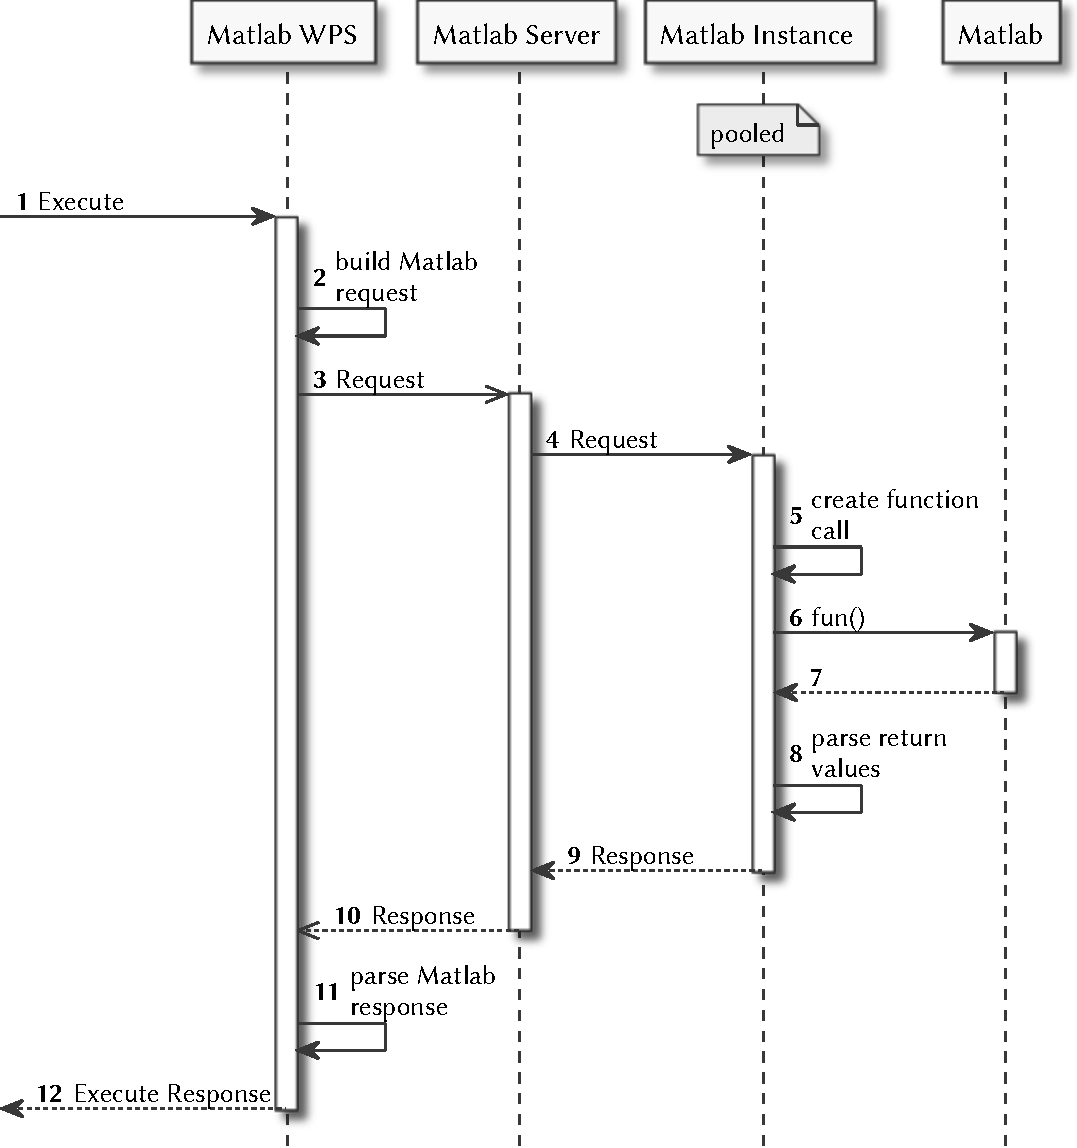
\includegraphics[width=.8\textwidth]{figures/sequence-diagramm-mwps.pdf}
		\caption{\label{fig:sd:mwps} Sequence diagram of the Matlab WPS.} %182x194
	\end{figure}
	\subsection{Lake-Analyzer WPS}
\section{Streaming WPS}
	\begin{itemize}
		\item the concept of streaming describes the sequential processing of data in contrast to random access processing
		\item processing takes place on small chunks instead of the complete dataset
		\item reduced processing resources needed to process smaller chunks
		\item reduced latency to see the output
		\item enables processing of indefinite large datasets (e.g. live analysis)
		\item widely known:
		\begin{itemize}
			\item media streaming (live/on-demand) video/audio streaming
			\begin{itemize}
				\item RTP and RTCP \citep{ietf:rfc3550}, RTSP \citep{ietf:rfc2326}, SIP \citep{ietf:rfc3261}
			\end{itemize}
			\item inter process communication
			\begin{itemize}
				\item pipes/sockets (local or network) \citep{buschmann1996pattern}
			\end{itemize}
		\end{itemize}
		\item the system should extends the traditional processing paradigm  (see Figure \ref{fig:streaming} (a))\dots
		\begin{itemize}
			\item \dots to enable input only streaming (see Figure \ref{fig:streaming} (b))
			\begin{itemize}
				\item input should be supplied subsequently
			\end{itemize}
			\item \dots to enable output only streaming  (see Figure \ref{fig:streaming} (c))
			\begin{itemize}
				\item intermediate outputs should be published as they come available
			\end{itemize}
			\item \dots to enable full input and output streaming  (see Figure \ref{fig:streaming} (c))
			\begin{itemize}
				\item input should be supplied subsequently
				\item intermediate outputs should be published as they come available
			\end{itemize}
			\begin{figure}[!htb]
				\centering
				% !TEX root = ../thesis.tex
\begin{tikzpicture}
	\scriptsize
	\tikzset{
	  ibox/.style = {draw, fill=string!50,  minimum width=4cm, minimum height=.6cm},
	  pbox/.style = {draw, fill=comment!50, minimum width=4cm, minimum height=.6cm},
	  obox/.style = {draw, fill=keyword!50, minimum width=4cm, minimum height=.6cm},
	  every node/.style={font=\sffamily},
	}
	\draw[>->] (-2.4,3.6) -- (11.4,3.6);
	%\draw[]   (-2.4,3.6) -- (-2.4, -6);
	\draw[>->] (-2.4, -6) -- (11.4, -6);

	\draw[dotted] (-2.0,-6) -- (-2.0,3.6);
	\draw[dotted] (-1.0,-6) -- (-1.0,3.6);
	\draw[dotted] (-0.0,-6) -- (-0.0,3.6);
	\draw[dotted] (1.0,-6) -- (1.0,3.6);
	\draw[dotted] (2.0,-6) -- (2.0,3.6);
	\draw[dotted] (3.0,-6) -- (3.0,3.6);
	\draw[dotted] (4.0,-6) -- (4.0,3.6);
	\draw[dotted] (5.0,-6) -- (5.0,3.6);
	\draw[dotted] (6.0,-6) -- (6.0,3.6);
	\draw[dotted] (7.0,-6) -- (7.0,3.6);
	\draw[dotted] (8.0,-6) -- (8.0,3.6);
	\draw[dotted] (9.0,-6) -- (9.0,3.6);
	\draw[dotted] (10.0,-6) -- (10.0,3.6);
	\draw[dotted] (11.0,3.6) -- (11.0,-6) node [below] {Time};

	\node [xshift=-1.5cm,yshift=2.4cm] {(a)};
	\node [ibox,yshift=3.0cm,xshift=1cm] (input1) {Input Upload};
	\node [pbox,yshift=2.4cm,xshift=5cm] (processing1) {Processing};
	\node [obox,yshift=1.8cm,xshift=9cm] (output1) {Output Download};

	\draw[dashed] (-2.4, 1.2) -- (11.4, 1.2);

	\node [xshift=-1.5cm,yshift=0cm] {(b)};
	\node [ibox,yshift= .6cm,xshift=1cm] (input2) {Input Stream};
	\node [pbox,yshift= .0cm,xshift=2cm] (processing2) {Processing};
	\node [obox,yshift=-.6cm,xshift=6cm] (output2) {Output Stream};

	\draw[dashed] (-2.4, -1.2) -- (11.4, -1.2);

	\node [xshift=-1.5cm,yshift=-2.4cm] {(c)};
	\node [ibox,yshift=-1.8cm,xshift=1cm] (input3) {Input Stream};
	\node [pbox,yshift=-2.4cm,xshift=5cm] (processing3) {Processing};
	\node [obox,yshift=-3.0cm,xshift=6cm] (output3) {Output Stream};

	\draw[dashed] (-2.4, -3.6) -- (11.4, -3.6);

	\node [xshift=-1.5cm,yshift=-4.8cm] {(d)};
	\node [ibox,yshift=-4.2cm,xshift=1cm] (input4) {Input Stream};
	\node [pbox,yshift=-4.8cm,xshift=2cm] (processing4) {Processing};
	\node [obox,yshift=-5.4cm,xshift=3cm] (output4) {Output Stream};
\end{tikzpicture}
				\caption{\label{fig:streaming}Four different types of processing data: (a) conventional processing, (b) streaming input data (c) streaming output data, (d) full input and output streaming \citep[based on][]{foerster2012live}.}
			\end{figure}
		\end{itemize}
		\item it should\dots
		\begin{itemize}
			\item \dots not rely on inefficient polling techniques
			\item \dots be deployable in a web browser environment
			\item \dots should rely on open and widely used standards
			\item \dots be as inter operable as possible with the existing WPS standard
			\item \dots allow not only sequential analysis but should also take dependencies between spatio-temporal features into account
			\item \dots be not dependent on the data format
			\item \dots should allow live analysis of data
			\item \dots should allow analysis of great data sets
			\item \dots should allow chaining
			\item \dots should allow to easily transform existing WPS processes into streaming processes
		\end{itemize}

		\item previous approaches \citep{foerster2012live}
		\begin{itemize}
			\item in strong correlation to media streaming \citep{ietf:draft-pantos-http-live-streaming-12}
			\item publishing data chunks in playlists
			\item client/wps polling playlist and fetches data chunks when they become available
			\item big overhead of continuous fetching (in what frequency?)
			\item asynchronous WPS Execute
			\item output playlist is transported by wps:ProcessStarted: ``A human-readable text string whose contents are left open to definition by each WPS server, but is expected to include any messages the server may wish to let the clients know. Such information could include how much longer the process may take to execute, or any warning conditions that may have been encountered to date. The client may display this text to a human user.''
			\item WPS standard highly constraining
			\item approach still stick to it for the sake of interoperability
		\end{itemize}
		\item previous approach is highly limited
		\begin{itemize}
			\item implementation only supports output streaming (\ref{fig:streaming}) (c))
			\item WPS/algorithm is splitting outputs $\Rightarrow$ highly format specific
			\item splitting of complex data is often a complex procedure that can not be automated
			\item each data items context important
			\item dependencies between data chunks can not be considered
			\item automatic splitting of e.g. features in a Feature Collection is highly format dependent
			\item browser based clients can not use streaming inputs
			\item they can not offer a file under a URL
			\item multiple outputs to stream?
			\item how to connect/coordinate multiple streamed inputs?
		\end{itemize}
		\item this approach\dots
		\begin{itemize}
			\item will fulfill all above mentioned requirements
			\item break out of the constraints imposed by the WPS standard
			\item while reusing terminology and technology of the WPS standard
			\item use modern web browser compatible technologies
		\end{itemize}
		\item create a messaging based architecture
		\item use WebSockets to accomplish true full-duplex streaming of data
		\item WPS is highly XML based: use widely known SOAP+WSA on top of WebSockets
	\end{itemize}

	\subsection{Protocol}
		\begin{itemize}
			\item A streaming process is identifiable instance of a streaming enabled process
			\item core of the Streaming WPS
			\item will receive inputs process them, and emit the outputs
			\item Starting of Streaming Process by executing a WPS process
			\item after starting of a streaming process the WPS execute will return immediately
			\item WPS outputs are identifier and WebSocket URL of the streaming process
			\item providing inputs and receiving outputs over WebSockets
			\begin{figure}[!htb]
				\centering
				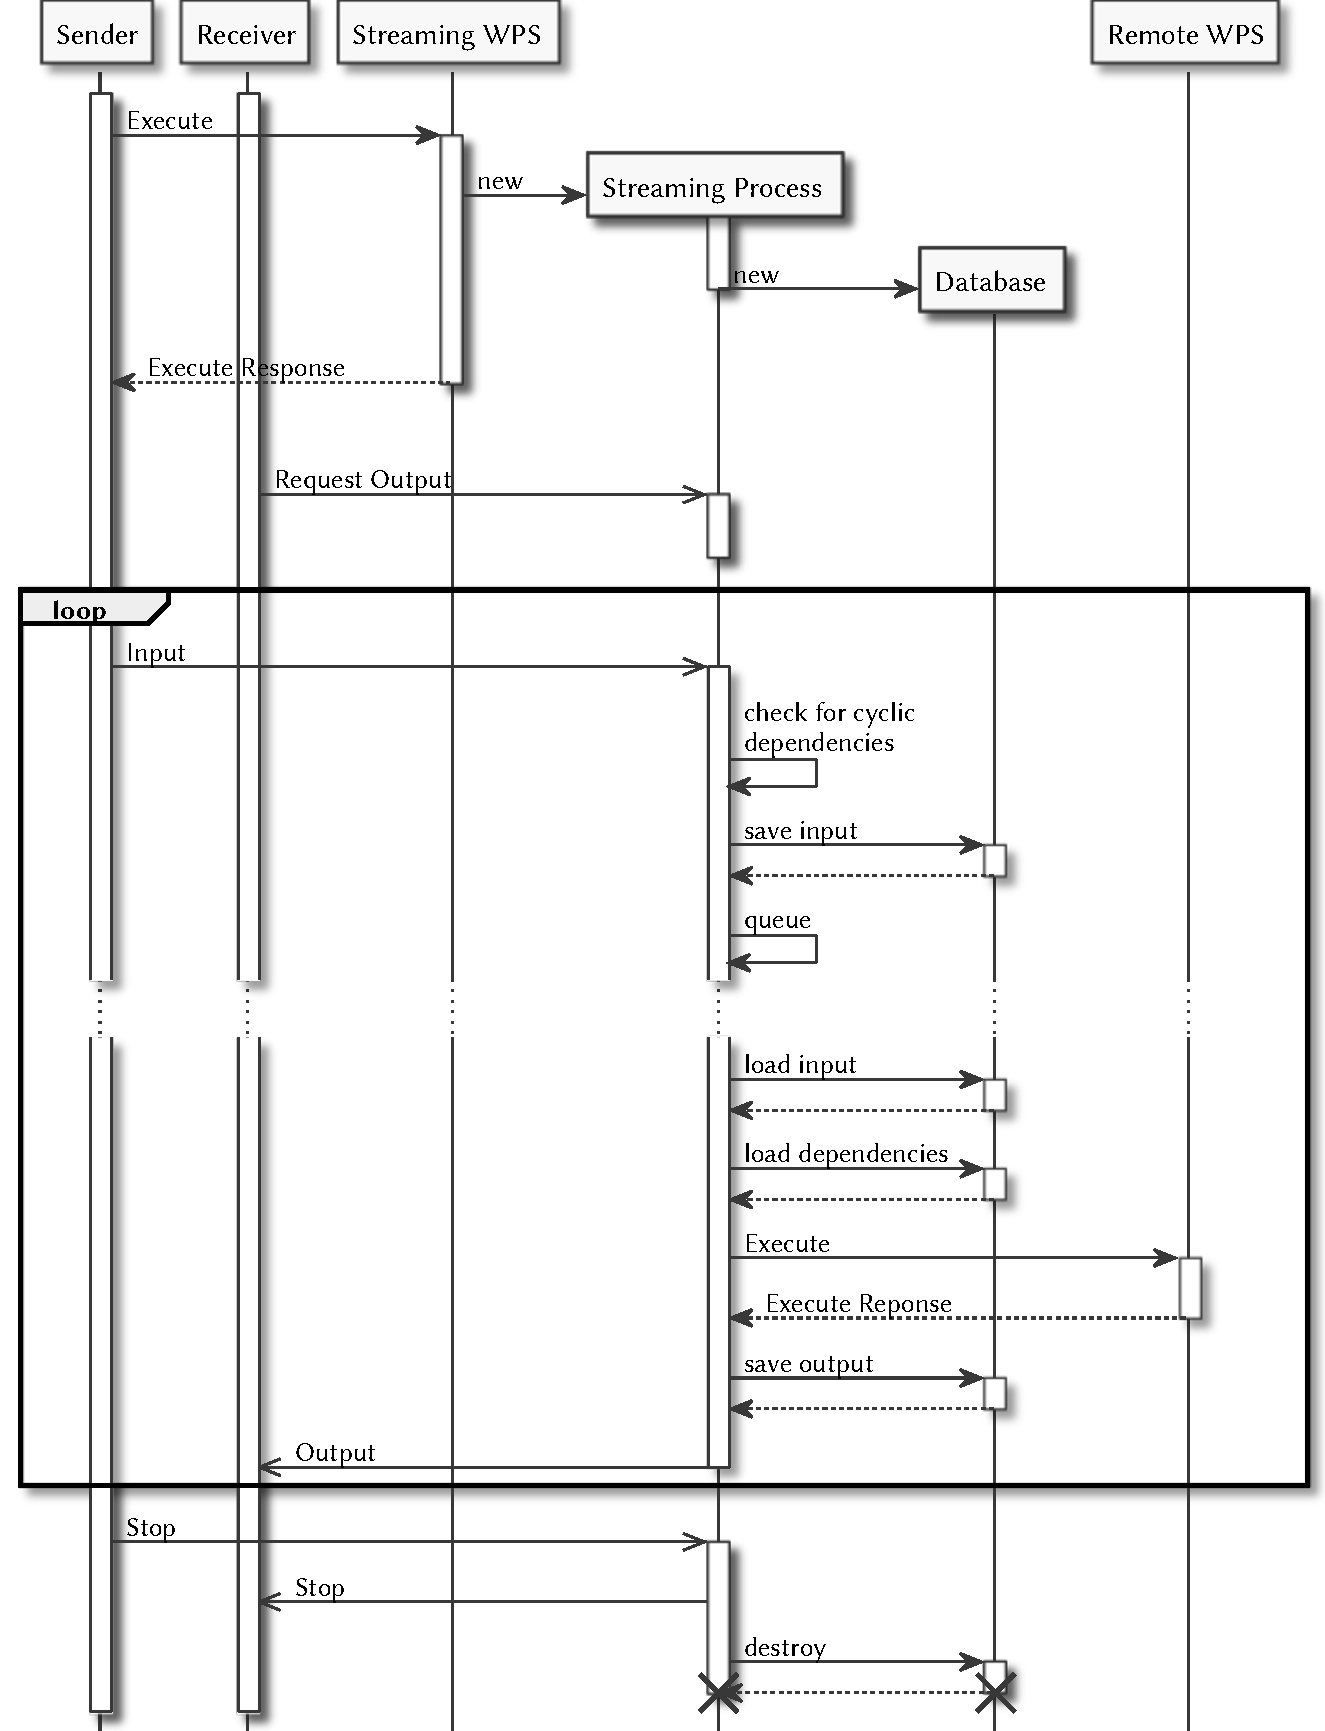
\includegraphics[width=.7868\textwidth]{figures/sequence-diagramm-swps.pdf} % 179x274
				\caption{\label{fig:sd:swps} Sequence diagram of the Streaming WPS.}
			\end{figure}
			\item detailed description (despicted in Figure \ref{fig:sd:swps})
			\begin{itemize}
				\item A client (Sender) issues a Execute to a streaming enables WPS process (step 1)
				\item the streaming WPS will instantiate a Streaming Process and a Delegate the will process data chunks (step 2 \& 3)
				\item The Streaming WPS returns the identifier and endpoint URL of the created Streaming Process in the ExecuteResponse
				\item One or more clients (which may also be the sender) connects to this endpoint URL and requests the outputs of the Streaming Process (step 5)
				\item One or multiple clients start sending chunks of data to the Streaming Process using Input Messages over WebSockets. The connection may stay open while feeding (step 6)
				\item the Streaming Process will check the inputs (especially whether the supplied input introduce a cycle (see section \ref{sec:stream:dependencies})) (step 8) and will enqueue them until they can be processed
				\item When the inputs can be processes the processing will be delegated to the delegate, which may or may not return a intermediate output  (step 9 \& 10)
				\item if theres is a intermediate result, the Streaming Process will push it to the listening clients (step 11)
				\item Steps 6--11 may be repeated until there are no more inputs available
				\item the sender will inform the Streaming Process by sending a stop message (step 12)
				\item the Streaming Process asks the delegate for a final result and will publish it, if is available (step 13--15)
				\item after this the Streaming Process will tell all listening clients that there will be no further outputs and will stop (step 18)
			\end{itemize}
			\item allows full input/output streaming: every input message results in a output message
			\item allows input only streaming: no intermediate outputs, only final output message
			\item allows output only streaming: even not depicted in the diagram, step 11 may be repeated
			\item multiple streaming inputs/outputs are possible
			\item encapsulated in a streaming iteration (1 InputMessage + (optional) OutputMessage)
			\item chaining of Streaming Processes possible
			\begin{itemize}
				\item can be implemented as a streaming Process that simply maps input to output names
				\item requires mediator between two streaming process that translates input messages into output messages
				\item see Figure \ref{fig:sd:chain}
				\item even simpler: delegate is a WPS process chain
			\end{itemize}
			\begin{figure}[!htb]
				\centering
				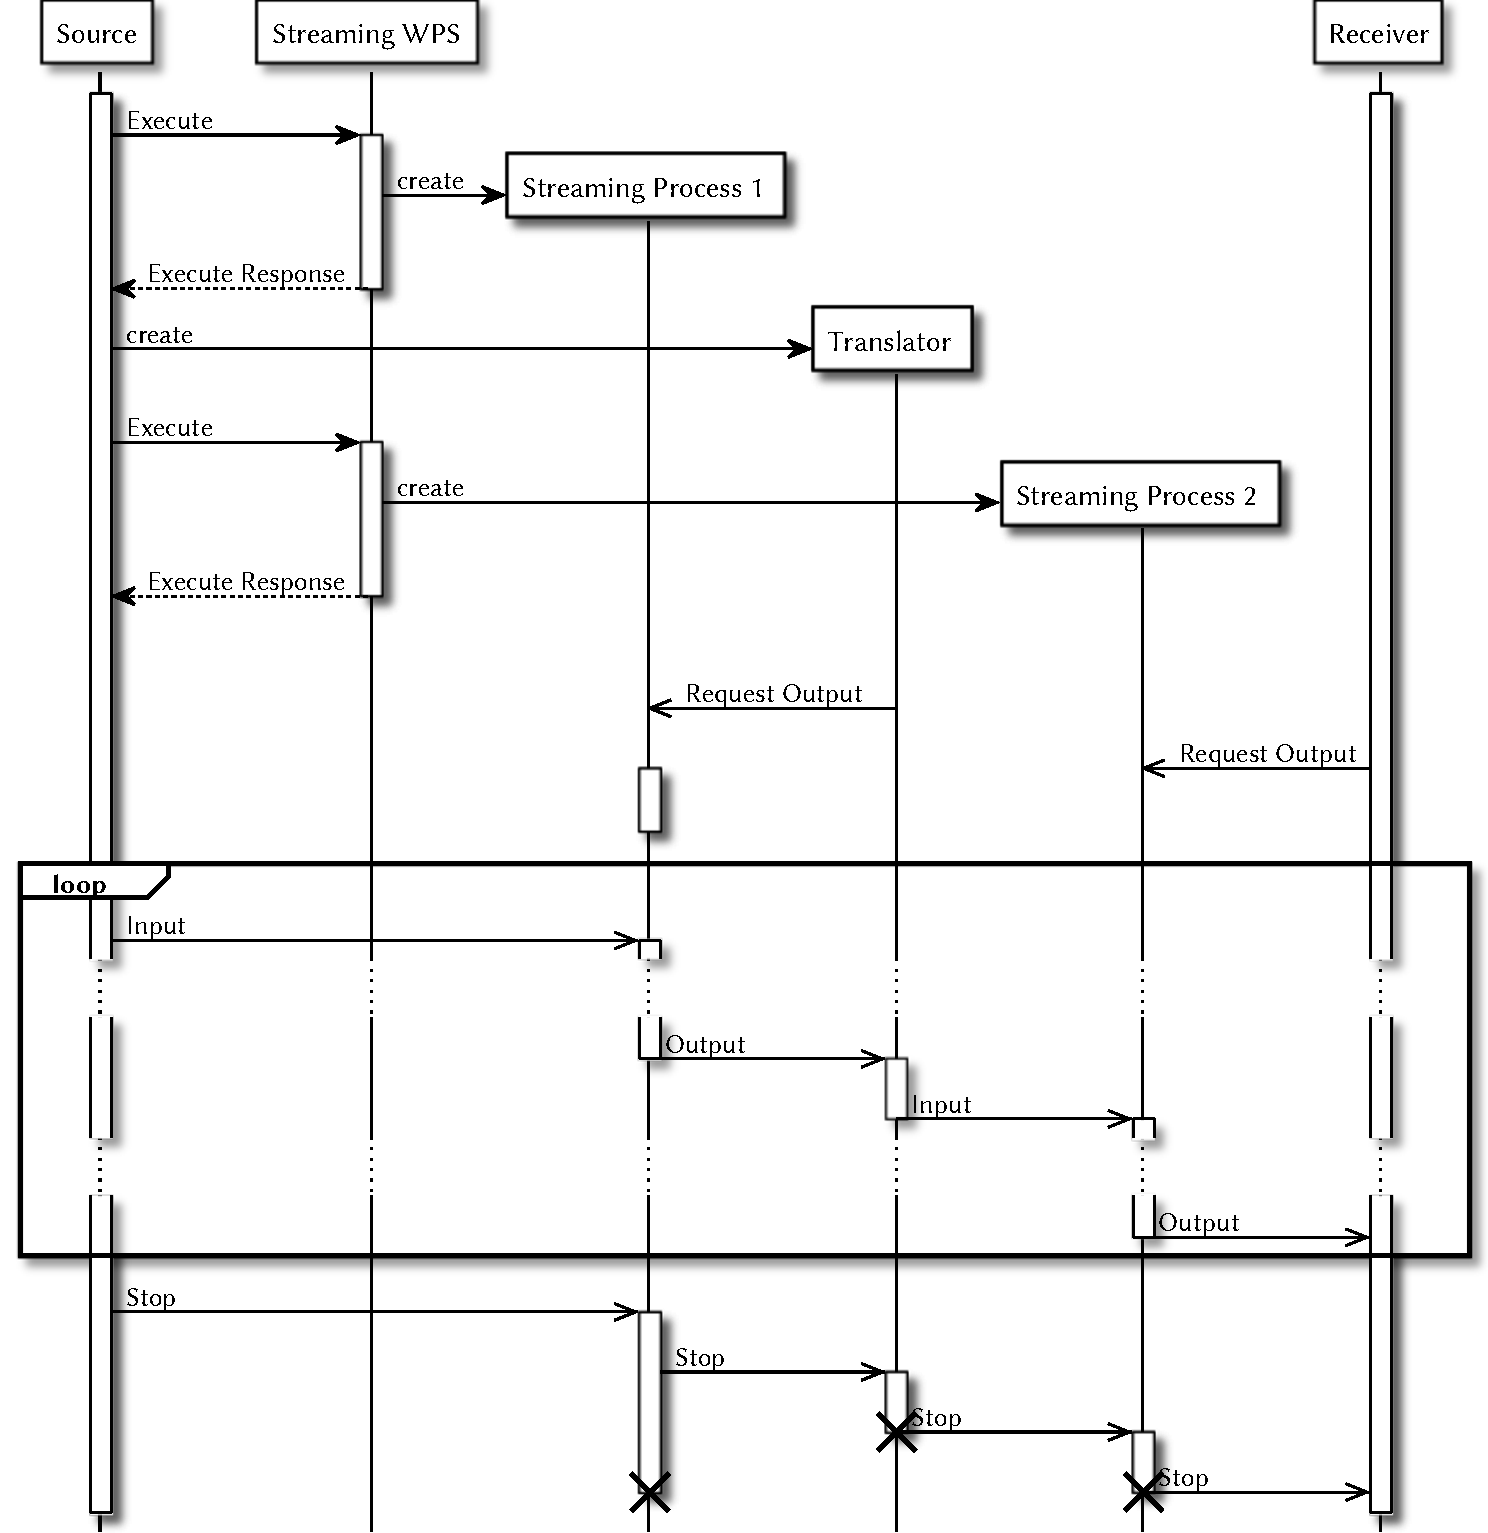
\includegraphics[width=\textwidth]{figures/sequence-diagramm-chain.pdf} % 179x274
				\caption{\label{fig:sd:chain} Sequence diagram of chaining two different streaming processes.}
			\end{figure}
		\end{itemize}
	\subsection{Input Types}\label{sec:streaming:input-types}
		\begin{itemize}
			\item three basic types of inputs
			\item difference when they are supplied
			\item and in which scope they are used
			\item all based on WPS data types
			\begin{itemize}
				\item Complex
				\item Literal
				\item Reference
				\item BoundingBox
			\end{itemize}
		\end{itemize}
		\subsubsection{Static Inputs}
			\begin{itemize}
				\item see Listing \ref{lst:streaming:input:static}
				\item inputs common to every streaming iteration
				\item supplied when starting the streaming process
				\item merged with streaming inputs and forwarded to delegate
				\item configuration parameters, etc.
				\item
			\end{itemize}
			\includecode[XML]{streaming-input-static.xml}{\label{lst:streaming:input:static}Example for a Streaming WPS static inputs.}
		\subsubsection{Streaming Inputs}
			\begin{itemize}
				\item see Listing \ref{lst:streaming:input:streaming}
				\item provided for a single streaming iteration
			\end{itemize}
			\includecode[XML]{streaming-input-streaming.xml}{\label{lst:streaming:input:streaming}Example for a Streaming WPS streaming inputs.}
		\subsubsection{Reference Inputs}\label{sec:stream:input:reference}
			\begin{itemize}
				\item see Listing \ref{lst:streaming:input:reference}
				\item references the output of a previous or upcoming streaming iteration as an input for this iteration
				\item used to model dependencies between iterations/features/etc.
				\item breaks out of the classical non-random access paradigm of streaming
			\end{itemize}
			\includecode[XML]{streaming-input-reference.xml}{\label{lst:streaming:input:reference}Example for a Streaming WPS reference input.}
		\subsubsection{Polling inputs}
			\begin{itemize}
				\item Not implemented inside the streaming WPS.
				\item what to do if multiple polling inputs are defined?
				\item how to define polling frequency?
				\item how to define notifications?
				\item better handled on client side (see Figure \ref{fig:sd:polling})
			\end{itemize}
			\begin{figure}[!htb]
				\centering
				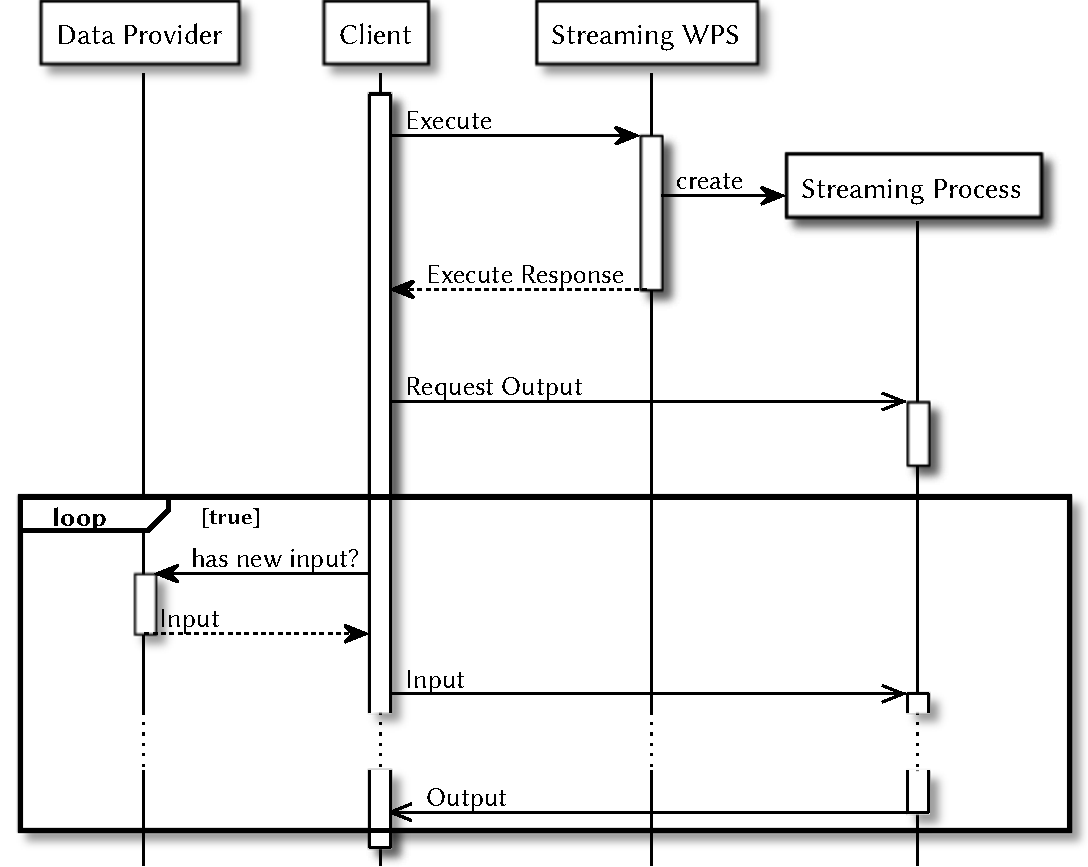
\includegraphics[width=.7868\textwidth]{figures/sequence-diagramm-polling.pdf}
				% 179x274
				\caption{\label{fig:sd:polling} Sequence diagram of polling inputs of the Streaming WPS.}
			\end{figure}
	\subsection{Messages}
		\begin{itemize}
			\item SOAP based message formats
			\item allows messages over an asynchronous protocol like WebSockets that has no concept of reply
			\item Messages:
			\begin{itemize}
				\item InputMessage
				\includecode[XML]{streaming-message-input.xml}{\label{lst:streaming:message:input}Example for a Streaming WPS input message.}
				\begin{itemize}
					\item used to provide inputs to a streaming iteration to the process
					\item comparable to a wps:Execute
				\end{itemize}
				\item OutputMessage
				\includecode[XML]{streaming-message-output.xml}{\label{lst:streaming:message:output}Example for a Streaming WPS output message.}
				\begin{itemize}
					\item used to send outputs of a streaming iteration to the client
					\item comparable to a wps:ExecuteResponse
				\end{itemize}
				\item OutputRequestMessage
				\includecode[XML]{streaming-message-output-request.xml}{\label{lst:streaming:message:output-request}Example for a Streaming WPS output request message.}
				\begin{itemize}
					\item used to request the outputs of a process from the process
					\item no direct counterpart in the WPS
				\end{itemize}
				\item ErrorMessage
				\includecode[XML]{streaming-message-error.xml}{\label{lst:streaming:message:error}Example for a Streaming WPS error message.}
				\begin{itemize}
					\item used to transport errors to the clients
					\item comparable to ows:ExceptionReport
				\end{itemize}
				\item DescribeMessage
				\includecode[XML]{streaming-message-describe.xml}{\label{lst:streaming:message:describe}Example for a Streaming WPS describe message.}
				\begin{itemize}
					\item used to request a description of a streaming process from the process
					\item comparable to DescribeProcess
				\end{itemize}
				\item DescriptionMessage
				\includecode[XML]{streaming-message-description.xml}{\label{lst:streaming:message:description}Example for a Streaming WPS description message.}
				\begin{itemize}
					\item used to describe a process to the client
					\item comparable to ProcessDescription
				\end{itemize}
				\item StopMessage
				\includecode[XML]{streaming-message-stop.xml}{\label{lst:streaming:message:stop}Example for a Streaming WPS stop message.}
				\begin{itemize}
					\item used to stop the streaming process, to indicate no further inputs will become available
					\item used to to notify any listening clients that no more outputs become available
					\item no direct counterpart in the WPS
				\end{itemize}
			\end{itemize}
		\end{itemize}
	\subsection{Dependencies}\label{sec:stream:dependencies}
		The definition of Reference Inputs in Section \ref{sec:stream:input:reference} implies a mechanism to resolve dependencies and to order the execution of streaming iterations. These are considered as tasks and can declare dependencies to other streaming iterations either by mapping an input to the output of another streaming iteration or by declaring a explicit dependency on another streaming iteration.

		Dependencies can be best modeled using a \ac{DAG}. A \ac{DAG} is a structure $D=(V, E)$ consisting of a set of vertices (or nodes) $V$ and edges (or arcs) $E$ where every edge $e\in E$ is a ordered pair $v_1 \rightarrow v_2$ with $v_1, v_2 \in V$. The distinct vertices $v_1,\dots,v_n\in V$ are called a path if for all successive vertices $v_i, v_{i+1}$ exists a edge $v_i \rightarrow v_{i+1} \in E$. A directed graph is called acyclic if there exists no path in $G$ with $v_1 = v_n$. A subgraph of a graph is the graph $G' = (V', E')$ with $V'\subseteq V$ and $E' = \{v_1 \rightarrow v_2 \in E | v_1, v_2\in V'\}$. Two subgraphs $G_1 = (V_1, E_1), G_2 = (V_2, E_2)$ are independent if $V_1 \cap V_2 = \emptyset$ and there exists no edge $v_1\rightarrow v_2\in E$ with $v_1\in V_1 \wedge v_2\in V_2$ or $v_2\in V_1 \wedge v_1\in V_2$.


		In a dependency graph, vertices represent a task, package or other entity that has dependencies and edges represent these dependencies ($v_1$ depends on $v_2$). Dependency graphs have to be acyclic as a cycle would introduce a cyclic dependency, that can not be resolved.

		\begin{figure}[!htb]
			\centering
			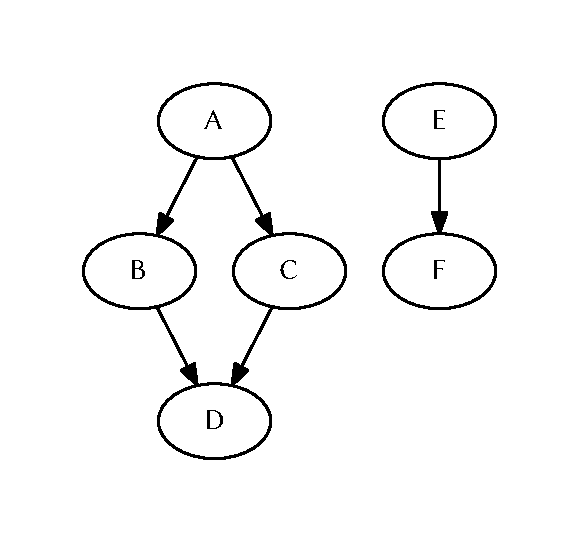
\includegraphics[width=.4474\textwidth]{figures/unordered-graph.pdf} % 98x92
			\caption{\label{fig:graph:unordered} Example for a dependency graph consisting of two independent subgraphs.}
		\end{figure}
		A system containing the tasks $A, B, C, D, E, F$ and the dependencies $A\rightarrow B, A\rightarrow C, B\rightarrow D, C\rightarrow D$ and $E\rightarrow F$ will result in a \ac{DAG} consisting of two independent subgraphs (see Figure \ref{fig:graph:unordered}).

		The execution order of a dependency graph can be derived from the topological ordering of the graph: a ``topological ordering, $ord_D$, of a directed acyclic graph $D = (V, E)$ maps each vertex to a priority value such that $ord_{D}(x) < ord_{D}(y)$ holds for all edges $x \rightarrow y \in E$'' \citep{pearce2007dynamic}, a possible execution order is the list of all vertices sorted by descending $ord_D$. The topological order of a \ac{DAG} can be computed using e.g. \ac{BFS} in linear time \citep{cormen2001introduction}. In most cases the topological ordering is not unique, Figure \ref{fig:graph:ordered} shows one possible execution order for the before mentioned graph.
		\begin{figure}[!htb]
			\centering
			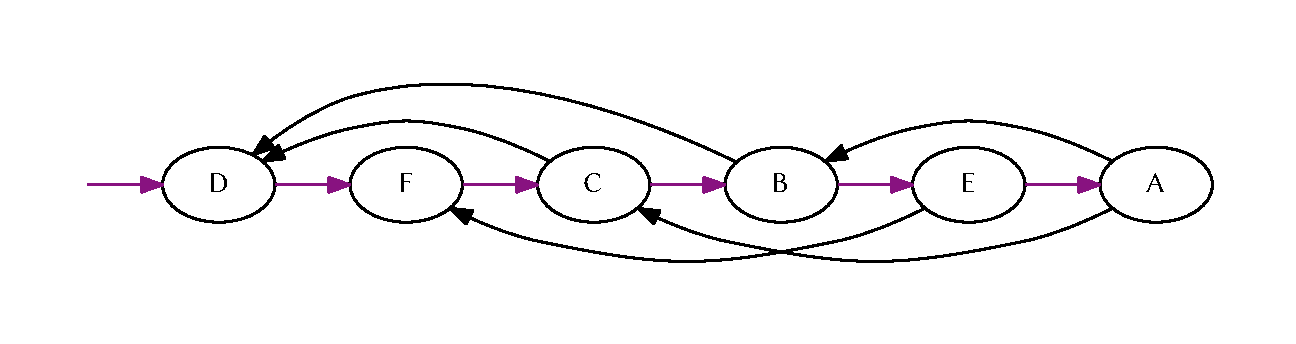
\includegraphics[width=1\textwidth]{figures/ordered-graph.pdf} % 219x58
			\caption{\label{fig:graph:ordered} Possible execution/topological order of the dependency graph in Figure \ref{fig:graph:unordered}. Black arrows represent dependence to another vertex, colored arrows the execution order.}
		\end{figure}

		In contrast to conventional dependency systems like package managers the Streaming \ac{WPS} can not operate on a static graph of dependencies but on a graph to which vertices and edges are added constantly. Conventional topological sorting algorithms have to recompute the ordering for every insertion from scratch which will have a big performance impact for the scenario of a great number of small streaming iterations. There exist few dynamic topological sort algorithms that will maintain the topological order across edge and node insertions and will only recompute the ordering if necessary.

		Most dependency graphs generated using the Streaming \ac{WPS} will probably consist of multiple independent subgraphs, no dependencies at all would be the most extreme example, or quite sparse graphs. For this the algorithm described by \citet{pearce2007dynamic} seems to be appropriate. Even it is theoretically it is inferior to other algorithms for dynamic topological sorting, it especially performs better on sparse graphs and on dense graphs only a constant factor slower than other algorithms \citep{pearce2007dynamic}.

		The actual implementation uses a \ac{DAG} only for a cyclic dependency check. Execution ordering is listener based to allow a better parallelization of streaming iterations.

	\subsection{Process Description}
		The conventional process description mechanism of the \ac{WPS} is not sufficient to describe streaming processes.

		It consists of a \texttt{DescribeProcess} request issued to the \ac{WPS} and the retrieval of one or more process descriptions of the specified process. These descriptions contain detailed descriptions of input and output parameters of the process and information about the supported formats, units of measurement or coordinate reference systems of each parameter. They also include details about allowed values, default value and multiplicity of input parameters \citep{ogc:wps}.

		Because the Streaming \ac{WPS} uses the \ac{WPS} interface only to start a Streaming Process and the \ac{WPS} interface does not provide any extension points for process descriptions, the \texttt{DescribeProcess} operation can only be used to describe the starting process, but not the input or output parameters of a streaming process.

		In case of generic processes, e.g. processes that delegate to other \ac{WPS} processes, information about input and output parameters is not even available prior to the execution of the streaming process. Furthermore input parameter cardinalities may change due to the use of static inputs. By this a valid input parameter for a delegate process may not be used in subsequent inputs because the maximal occurrence of the parameter is already exhausted using static input parameters. By this a process description for a streaming process will always be instance specific and can not be generated by the associated \ac{WPS} process.

		With knowledge of the delegate process a client may has enough information to facilitate the streaming process but for other streaming process there is no way for a generic client to know the input parameters of the process.

		To compensate this shortcoming a method is needed to describe a Streaming Process instance at runtime.
	\begin{itemize}
		\item WPS Process description
		\begin{itemize}
			\item not extendable
			\item no subsequent inputs/outputs
		\end{itemize}
		\item Streaming inputs can not be described there
		\item descriptions may change with different static inputs
		\item not important when delegating but other processes need to describe them self as well
		\item subsequent outputs/final result
		\item description runtime
		\item description of instances
		\item currently only a boolean flag/no differentiation between final/subsequent
	\end{itemize}

	\subsection{Implementation}
	\begin{itemize}
		\item based on the 52°North WPS
		\item includeable module
		\item default implementation uses another WPS process as delegate
	\end{itemize}
	\subsection{Client Implementation}
	\begin{itemize}
		\item small JavaScript library
		\item abstracts the message generation and WebSocket interaction
		\item may be used to start generic delegation processes
	\end{itemize}
	\subsection{Streaming Lake-Analyzer WPS}
	\begin{itemize}
		\item simple application of the Streaming WPS and Matlab WPS
		\item LakeAnalyzer may need further adjustments to allow live analysis
		\item remove down sampling code
		\item operate on single point in time
		\item etc
	\end{itemize}
	\subsection{Limitations}
	\begin{itemize}
		\item No input/output conversion
		\item Only default format is requested from delegate
		\item process will not fail fast in under every condition
		\begin{itemize}
			\item inputs first are checked at execution time
		\end{itemize}
		\item receivers are only provided with upcoming
		\begin{itemize}
			\item no replay queue
		\end{itemize}
	\end{itemize}
\section{Future Work}
\section{Conclusion}